\chapter{Estado del arte}

 En este capítulo se revisarán la literatura relacionada con la Agricultura inteligente, así como las plataformas comerciales existentes.
%Si queremos ponernos en situación respecto a este trabajo y a las empresas, primero tenemos que explicar un concepto que surgió en los últimos años, la Agricultura 4.0 o Agricultura Inteligente.

% \section{La revolución verde}

% \section{Internet of Food \& Farm}

\section{Agricultura inteligente}
% Puedo hacer subsecciones de la lista y extenderlo más del articulo incluido en el doc%
%https://agrospray.com.ar/blog/agricultura-4-0/%



La agricultura inteligente \cite{agricultura-40}, o agricultura 4.0 se basa en la recopilación y análisis de datos sobre el campo, con el objetivo de mejorar la calidad de los cultivos y reducir las consecuencias en el medio ambiente.

Esto es posible con el uso de las nuevas tecnologías. Los diferentes robots, sensores, software, etc, son capaces de realizar tareas agrícolas en menos tiempo que el ser humano y con mejor resultados.

Ejemplos de tecnología utilizada en la agricultura:

\begin{itemize}
    \item \textbf{Sensorización ambiental}, referente al uso de sensores, obteniendo la información en tiempo real para optimizar mejor los recursos.
    \item \textbf{Uso de drones y teledetección}, con el objetivo de tomar fotos para analizar el estado, o incluso pulverizar un producto en cultivos.
    \item \textbf{Sistemas predictivos}, permitiendo la anticipación a las diferentes condiciones meteorológicas en las próximas horas o días.
    \item \textbf{Inteligencia artificial}, para tomar decisiones o realizar recomendaciones en base a los datos procesados.
    
\end{itemize}

Aparte de estos puntos, podemos destacar unos de los temas tocados en este proyecto, la robotización.

\subsection{Robots en el sector}


En \cite{revista-agraria} hay un artículo donde se comenta que los desarrolladores actualmente están trabajando en máquinas autónomas capaces de realizar tareas como las siguientes:

\begin{itemize}
    \item \textbf{Desbrozar}. Eliminar las malas hierbas mediante el reconocimiento de imagen con una cámara y expulsar dosis de herbicida según la mala hierba y el tamaño
    \item \textbf{Recogedor}. Realizar una recolecta del cultivo mediante la utilización de brazos robóticos, analizando la madurez de este.
    \item \textbf{Abonador}. Analiza el tamaño y color de las hojas de cada planta, aplicando una dosis de fertilizante según la necesidad de este.
\end{itemize}

Todas estas máquinas se podrían comunicar entre ellas, siendo controladas por un operador o trabajando de manera autónoma con ciertos horarios. Estas podrían ser utilizadas en los siguientes escenarios que se explicarán a lo largo del documento.

\section{Sistemas utilizados en la industria}

Esta parte ha sido una de las más complicadas de escribir, ya que no es fácil saber que tecnologías utilizan estas empresas debido a que las explicaciones realizadas en sus respectivas páginas web son muy genéricas del estilo: \textit{Consulta tus datos en tiempo real desde cualquier dispositivo.}

Como se ha visto en el anterior apartado, la mayoría de empresas tienen en común: \textbf{sensores} y \textbf{actuadores}, los cuales se van a agrupar de ahora en adelante como \textbf{nodos}.

Estos son la base del sistema, ya que son los \textbf{productores} de los datos a tratar, y de los cuales se obtiene la mayoría de la información. A continuación voy a realizar una lista de los algunos tipos que se deberían contemplar en el diseño, pudiendo ser estos aún más según las necesidades:

\begin{itemize}
    \item Temperatura del suelo, para ver el estado de la planta
    \item Humedad, tanto fuera como dentro del invernadero
    \item Estado hídrico del cultivo, para controlar los patrones de riego
    \item Velocidad del Viento
    \item Dirección del viento
\end{itemize}

Estos productores sirven para que los actuadores hagan ciertas funciones. Pero además hay otros actuadores que quizás no necesitan la información de estos sensores como un robot de transporte, brazo robot de recolecta, o algo más factible como los drones para realización de fotografías. Algunos actuadores que si utilizan la información de los productores son:

\begin{itemize}
    \item \textbf{Ventanas}, para transpirar y cambiar el aire de dentro
    \item \textbf{Calefactores}, para aumentar la temperatura
    \item \textbf{Humidificadores}, necesario en climas secos
    \item \textbf{Tuberías para riego}, permitiendo la circulación del agua
    \item \textbf{Pantallas térmicas}, con el objetivo de mantener fresco el terreno en días de mucho calor
    \item \textbf{Destratificadores}, ciclando el aire del interior, ya que el aire frío suele quedarse a nivel del suelo y el caliente tiende a subir.
\end{itemize}

En el siguiente conjunto de figuras \ref{fig:imagenes-actuadores} hay mostrados algunos de los actuadores menciondos

\begin{figure}[h]
\begin{subfigure}{\textwidth}
\centering
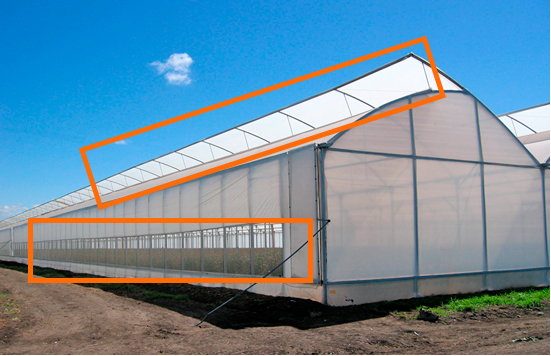
\includegraphics[width=0.9\textwidth, height=6cm]{img/03-Ventana.png}
%https://www.agroprecios.com/noticias.php/noticias/3371-mas-del-90-de-los-agricultores-de-almeria-controlan-manualmente-las-ventanas-del-invernadero?len=1
\caption{Ventanas (Imagen de la web de agroprecios)}
\label{fig:ventanas}
\end{subfigure}
\begin{subfigure}{\textwidth}
\centering
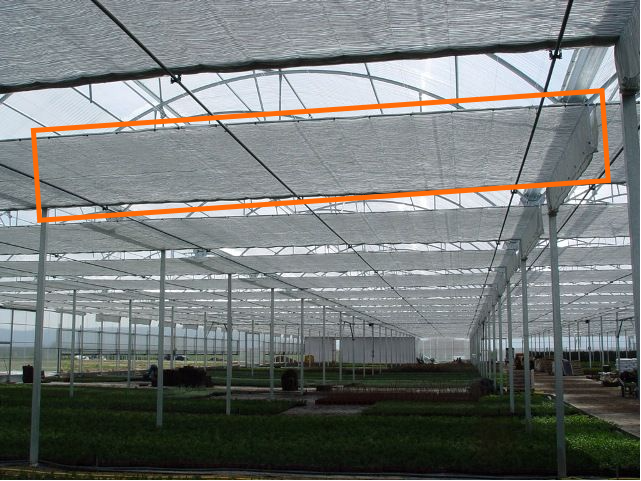
\includegraphics[width=0.9\textwidth, height=6cm]{img/03-PantallaTermica.png}
% https://fertri.com/accesorios-y-componentes/pantallas-termicas/
\caption{Pantallas térmicas (Imagen de la web fertri.com \cite{fertri})}
\label{fig:pantallas-termicas}
\end{subfigure}

\begin{subfigure}{\textwidth}
\centering
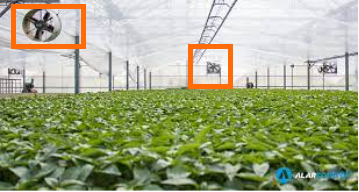
\includegraphics[width=0.9\textwidth, height=6cm]{img/03-Destratificador.png}
% https://fertri.com/accesorios-y-componentes/pantallas-termicas/
\caption{Destratificador (Imagen de la web de Alarcontrol \cite{alarcontrol-sl})}
\label{fig:destratificador}
\end{subfigure}

\caption{Imágenes de diferentes actuadores}
\label{fig:imagenes-actuadores}

\end{figure}

\clearpage

Por lo tanto, tras estudiar los diferentes productos desplegados por las empresas que las empresas utilizan, el autor de este trabajo propone dividir las soluciones actuales en dos grupos: \textbf{centralizadas} o \textbf{descentralizadas}.

% Aclaración de centralizado y descentralizado

\subsection{Despliegues centralizados}

En este caso, todo está conectado a un nodo que orquesta toda la plataforma.
Un ejemplo de empresa que utiliza este despliegue es Alarcontrol S.L. \cite{alarcontrol-sl}. 

La figura \ref{fig:despliegue_centralizado} nos da una idea de cómo es esta implementación. Esta consta de un panel central, donde un dispositivo gestiona todas las tareas, recopilando los datos de los diferentes sensores colocados en puntos estratégicos del terreno y conectados cada uno mediante un cable a la placa central.

\begin{center}
    \centering
    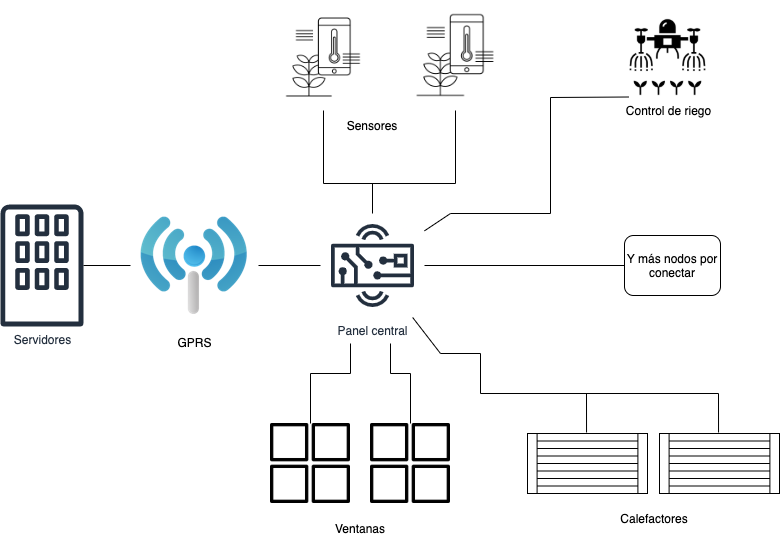
\includegraphics[width=\textwidth]{img/02-DespliegueCentralizado.png}
    \captionof{figure}{Despliegue centralizado (Elaboración propia)}
    \label{fig:despliegue_centralizado}
\end{center}

En el panel central se podrían encontrar diferentes botones para diversas acciones, además de una réplica de este dentro del invernadero para gestionar otros actuadores más cercanos, como ventanas o calefactores.

Por último tiene conexión \ac{GPRS}%, que es lo que venimos a conocer como cobertura móvil
. 
Esta la utiliza para transmitir los datos a un servidor central y que el usuario desde el móvil pueda visualizarlos.


Una posible desventaja de este servicio es la disponibilidad, ya que en el caso de que falle el %ese mencionado anteriormente 
gestor central no se podría disponer de ningún dato generado ni de los actuadores. Esto es debido a que no hay un sistema de respaldo, por lo tanto por muchas pruebas que se le hayan realizado, podría fallar.

\subsection{Empresas con despliegues descentralizados}

A diferencia del anterior, al ser descentralizado, no todo es gestionado por un único dispositivo, si no que podemos encontrar varios. Ejemplos de empresas que utilizan este diseño son Nazaríes \cite{nazaries} y Hortisys \cite{hortisys}.

Este sistema distribuye las tareas en más nodos, que poseen conectores genéricos para enchufar diferentes dispositivos, en función requiera el usuario. En el caso de la empresa Nazaríes, los nombra como \textit{Dataloggers}, que viene a ser recopilador de datos. Un ejemplo de este dispositivo lo podemos visualizar en la siguiente figura:

\begin{center}
    \centering
    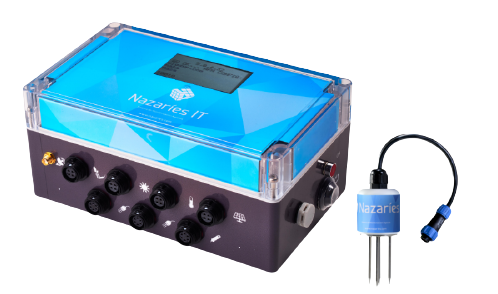
\includegraphics[width=0.5\textwidth]{img/03-Datalogger-Nazaries.png}
    \captionof{figure}{Datalogger GPRS junto a un sensor (Imagen de Nazaries \cite{nazaries})}
    \label{fig:datalogger-nazaries}
\end{center}

Como podemos observar, en el pie de la figura se hace referencia de GPRS. Esto es debido a que hay diferentes tipos de recopiladores de información según su conexión o visualización de datos: bluetooth, sigfox \cite{sigfox} o mostrados en un terminal.

% Añadir descripciones de bluetooth, sigfox, terminal?

Esto significa que trabaja de manera similar al despliegue centralizado, lo único que divide la carga, ya que diferentes nodos se encargan de recopilar esta información.

Pero esto también plantea un problema, y es que si uno de esos nodos se rompe, todos los datos que recopilaba no pueden ser visualizados.

Este supuesto fallo sería menos grave que en el caso anterior, ya que en el otro la plataforma entera dejaría de funcionar, y en este conlleva la pérdida de información del número de sensores conectados a este \textit{datalogger}.

\section{Tecnologías para publicación suscripción} \label{tecnologias_a_usar}

En el articulo de la bibliografía \textit{Meeting iot platforms re-quirements with open pub/sub solutions} \cite{pub-sub-solutions}, se define el patrón pub-sub como un \ac{MoM} que proporciona una comunicación distribuida, asíncrona entre productores y consumidores de mensajes. Este patrón presenta tres tipos principales de desacoplamiento que lo hacen especialmente adecuado para los despliegues de \ac{IoT} a gran escala:

\begin{itemize}
    \item Los productores de mensajes (publicadores) y los consumidores (suscriptores) están desacoplados en el tiempo, es decir, no tienen que estar conectados al mismo tiempo.
    \item Los mensajes no se dirigen a un consumidor en específico, si no a una dirección simbólica (canal, tópico)
    \item La mensajería es asíncrona y no se bloquea.
\end{itemize}

Uno de los elementos fundamentales de los sistemas pub/sub es la correspondencia entre productores y suscriptores, que puede basarse en distintos tipos de filtrado, principalmente de temas o contenidos. Este filtrado suele ser realizado por múltiples intermediarios de mensajes dedicados.

Tras la introducción de este sistema, se va a realizar una breve descripción de algunas tecnologías que lo aplican y cuál ha sido escogida para este proyecto.

\subsection{RabbitMQ}

RabbitMQ \cite{rabbitmq} es un software message-broker (negociador de mensajes) originalmente implementado con el protocolo \ac{AMQP}, con soporte a otros protocolos como por ejemplo \ac{STOMP} y \ac{MQTT}. Tiene la ventaja de que es independiente al lenguaje utilizado, y puede ser desplegado en .NET, Python, PHP, Ruby, etc.

Esta tecnología empezó como sistema de colas, por ello la parte de MQ en el nombre. Debido a esto, la implementación que realiza pub-sub está construida sobre este sistema. Esto puede ser que no sea lo más eficiente respecto a otra alternativa que su diseño si sea basado en el modelo de pub-sub. Además utiliza brokers (intermediarios entre pub-sub), haciendo que la conexión no sea directa y surja otro punto de posible fallo.

\subsection{Apache Kafka}

Kafka \cite{kafka} es un sistema de mensajería tipo pub-sub, escrito en lenguaje Scala, siendo escalable, duradero y tolerante a fallos. Es utilizado por empresas como Linkedin, Yahoo, Twitter y otras.

Su principal uso destaca en el análisis a tiempo real, pero se puede utilizar para supervisión, reproducción de mensajes, agregación de registros, recuperación de errores y el seguimiento de la actividad de un sitio web.

Pero para uso en IoT donde los dispositivos están conectados a un centro de datos o a la nube, Kafka no es idónea ya que necesita bastante configuración. Además hay una serie de puntos que no la hacen idonea para este entorno:
\begin{itemize}
    \item No soporta una enorme cantidad de tópicos
    \item Los brokers necesitan estar directamente direccionados por los clientes
    \item Algunas de las claves de las funcionalidades de IoT no están presentadas en Kafka, como por ejemplo \textit{keep alive}. Esta hace referencia al historial de datos a mantener en la red.
    \item Es necesario una conexión estable TCP, no muy presente en estos entornos, haciendo que los dispositivos gasten recursos en la reconexión.
\end{itemize}

\subsection{ROS2}

ROS2 \cite{ros2} es un conjunto de herramientas software utilizadas principalmente para la creación de estos robots. Empresas como BMW de automoción o la NASA utilizan ROS en algunos de sus proyecto. Por destacar, es utilizado en el Robonaut 2 \cite{robonaut}.

Las características principales que surgieron tras su desarrollo fueron:

\begin{itemize}
    \item Sistemas en tiempo real, para diferentes tratamientos de datos
    \item Equipos de múltiples robots, pudiendo comunicarse entre ellos para diferentes tareas
    \item Para conexiones no ideales, es decir, gestionando perdidas o delay de una red WiFi de poca calidad
\end{itemize}


Por defecto, ROS2 utiliza \ac{DDS} \cite{dds-omg} como middleware para la comunicación. 
DDS está orientado a usarse en computación distribuida implementando el patrón de esta sección, publicador-subscriptor. Permite el manejo de los mensajes de manera transparente sin la necesidad de la intervención del usuario, incluyendo algunas funciones como quien debería recibir el mensaje, donde están situados los consumidores o que pasaría si el mensaje no pudiese ser enviado. Además DDS soporta diferentes lenguajes como C, C++, Java o Python gracias a la \ac{APIs} disponibles. Esto permite que diferentes dispositivos, con sistemas operativos o lenguajes distintos puedan comunicarse. Esto viene a ser conocido como interoperabilidad.

\begin{center}
    \centering
    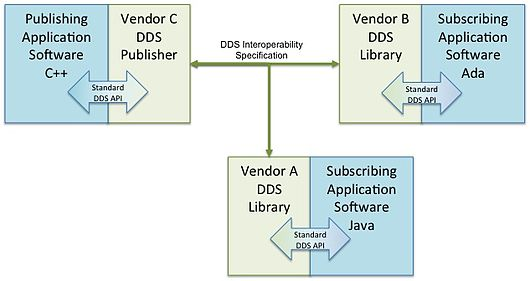
\includegraphics[width=0.5\textwidth]{img/03-DDS-Interoperability.jpeg}
    \captionof{figure}{OMG DDS interoperabilidad}
    \label{fig:dds-wiki}
\end{center}

El escenario mostrado en la figura \ref{fig:dds-wiki} se puede obtener del artículo \cite{dds-omg}. En el se explica la interoperabilidad del protocolo utilizado para la conexión de los diferentes dispositivos.

Tras explicar algunos conceptos y funcionalidades sobre DDS, caracterizar que no existen brokers en algunas de sus implementaciones, ya que utiliza un protocolo multicast basado en descubrimiento de dispositivos (intermediarios entre pub-sub). Además simplifica el despliegue, minimiza la latencia, maximiza la escalabilidad y aumenta la fiablilidad. Por tanto es idóneo para aplicaciones IoT que requieren de una arquitectura duradera y fiable.

Respecto a ROS 2, utiliza un middleware para ser independiente a la implementación de DDS utilizada, además de ofrecer una API para los diferentes lenguajes de programación soportados. Esta información se puede visualizar en la siguiente imagen:


\begin{center}
    \centering
    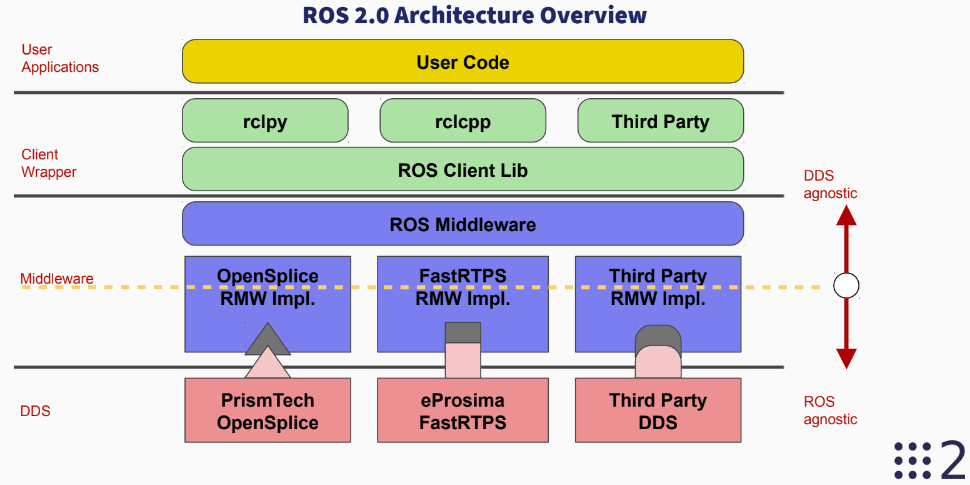
\includegraphics[width=\textwidth]{img/03-ROS2-Middleware.png}
    \captionof{figure}{Capas disponibles con ROS 2}
    \label{fig:ros-layers}
\end{center}

En la figura \ref{fig:ros-layers} se puede observar las capas de la API que ofrece ROS 2.

Por último, ROS2 es compatible con múltiples implementaciones de DDS, como de eProsima's Fast DDS \cite{fastdds}, RTI's Connext DDS \cite{connextdds} y Eclipse Cyclone DDS \cite{cyclonedds}. Por defecto, ROS2 utiliza el producto de eProxima's.

Cabe destacar que para poder utilizar ROS en microcontroladores, es necesario el uso de microROS. Este se diferencia de que la implementación es realizada en C/C++, además que deberá situarse en una capa por encima que actúe como sistema operativo, como \ac{FreeRTOS}.

El diagrama de comunicación y de capas se puede visualizar en la siguiente imagen:

\begin{center}
    \centering
    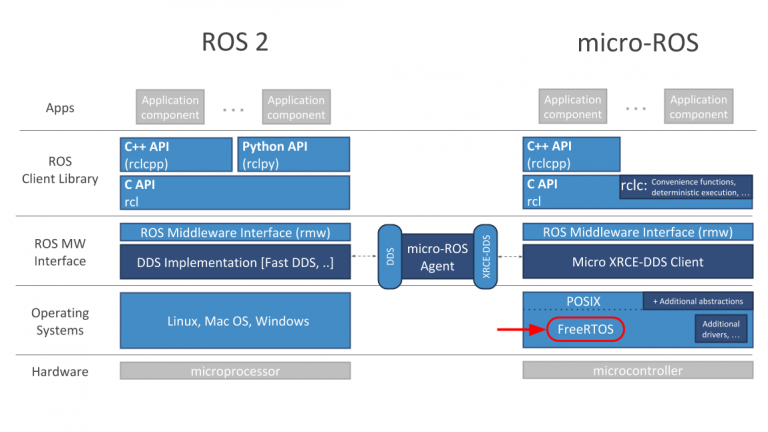
\includegraphics[width=\textwidth]{img/02-micro-ros.png}
    \captionof{figure}{Comparación estructura ROS2 y microROS}
    \label{fig:ros2-microros}
\end{center}

Como se puede observar en \ref{fig:ros2-microros}, en el centro esta situado una figura que pone micro-ROS Agent. Este es el encargado de comunicar la parte de DDS (la parte del middleware de ROS) generada por el microcontrolador con las diferentes implementaciones de DDS que existan en la red.